% !Mode:: "TeX:UTF-8"

\chapter{恶意代码家族画像构建方法}[Example]
主要介绍恶意代码家族画像以及对应的构建
将文本分类作为恶意代码家族画像的一部分。
\section{引言}[Number]

在第3章中描述了如何根据恶意代码动态行为报告来构建恶意代码个体行为画像。
本章在恶意代码个体画像的基础上结合恶意代码的文本报告来构建恶意代码的家族画像。

恶意代码的家族指的是具有同样的目的以及攻击手段的恶意代码的集合,
一般同一家族的恶意代码都是某一恶意代码的变体,虽然有着不同的改进版本,
但是最终的目的和关键行为还是相似。
而仅仅研究恶意代码个体的画像是不足以发现其家族的行为规律的,
因此提出了恶意代码家族画像的研究。

近些年来恶意代码的抗检测性越来越强,加密混淆等方法有效降低了静态分析的准确性。
随着动态分析的广泛应用,恶意代码为了躲避动态分析,会添加大量无用行为来进行混淆,
其中主要是添加一些正常的行为\cite{RN33}。
因此只有恶意代码的动态行为不足以进行恶意代码家族的画像的构建,还需要准确的标签辅助。
本章结合了恶意代码个体的动态行为以及恶意代码的文本报告来构建恶意代码的家族画像。
互联网上有着大量的恶意代码文本资源,例如恶意代码的APT报告或者博客等都在一定程度上描述了恶意代码家族的能力,
本章主要通过恶意代码文本中的句子进行分类,判断该句子描述了恶意代码的哪种能力,从而了解文本对应家族所具有的能力。


目前对于这些恶意代码文本资源的利用工作还很少。
其中主要有几个难点,一是恶意代码文本具有领域特性,其中包含大量的专业名词,
通用的自然语言处理模型在其中表现效果并不好;
二是数据集的匮乏。目前已标注的公开数据集十分稀少,只有个别的数据可用,而且数据量也十分小。


本章对基于恶意代码个体动态行为以及恶意代码文本信息的家族画像构建做出了尝试,
对现有的数据集进行了改进,提出了恶意代码领域的文本处理方法获得了良好的效果,构建了恶意代码家族画像。



\section{主要任务介绍}
本章的主要任务是通过对恶意代码文本中的句子进行分类,来判断该句子描述了何种恶意能力。
由于文本中的大部分句子没有直接描述恶意能力,因此需要将任务拆分成两个子任务。
一是判断该句子是否描了恶意代码的恶意能力;
二是判断描述了恶意代码能力的句子描述了何种能力。


子任务一是一个二分类任务,用于判断文本中的句子是否描述了恶意代码的能力,是对句子的初步筛选。
如表4-1中所示,恶意代码文本中描述了恶意代码能力的句子与无关的句子的比例接近1:4,
如果不进行初步的筛选,而直接将无关句子归为一类会导致数据集分布出现一类占比特别大,其余的占比较小的情况。
因此子任务一的存在是有必要的。
子任务二是对句子进行多分类,判断句子描述了何种恶意代码能力。

在获得了恶意代码家族的文本信息之后,
需要结合恶意代码个体的行为以及文本中给出的能力,来构建恶意代码家族的画像,
通过这个画像可以给出家族的代表性的行为以及对应的能力,对恶意代码的研究和防御有着较大的价值。


\section{恶意代码文本数据处理}
\subsection{数据集相关介绍}
恶意代码的文本报告主要包括恶意代码的高持续性威胁报告(Advanced Persistent Threat,APT)、
杀毒软件厂商的报告以及安全相关的博客等。
这些报告会对一些恶意代码家族以及安全相关的问题进行描述,其中就包括了恶意代码家族的能力信息。
目前已标注的恶意代码报告数据集很少,目前只有 SemEval-2018 Task8\cite{RN100}中给出的 MalwareTextDB 数据集较为完善,
因此本章以该数据集为基础,根据任务需求对其进行修改。

MalwareTextDB 中对 85 个 APT报告进行了标注, 
其中标注采用了MAEC(Malware Attribute Enumeration and Characterization)词汇表来进行文本标注。
该数据集主要有四个相关的子任务:(1)判断句子的恶意代码相关性,该任务是后续的基础,后续任务都是在恶意代码相关
的句子上进行的。(2)提取恶意代码相关句子中的实体,主要有Action、Subject、Object以及Modifier四类。(3)判断实体
之间的关系,主要有SubjAction,ActionObj,ActionMod以及ModObj四类。(4)判断Action实体对应的行为名称、能力、
战略目标和战术目标属性。

本章的任务一与SemEval-2018 Task8中的任务一一致,直接采用该数据,其具体分布如表~\ref{tab:relative}~
\begin{table}[htb]
	\renewcommand{\arraystretch}{1.3}
	\caption{恶意代码相关性判断任务数据集分布}
	\label{tab:relative}
	\vspace{0.5em}\centering\wuhao
	\begin{tabular}{c c c c}
		\toprule  & 相关句子数量 & 非相关句子数量 & 总句子数量  \\
		\midrule[1pt] 
		Train & 2204 & 7220 & 9424 \\
		Dev & 79 & 1134 & 1213 \\
		Test & 90 & 528 & 618 \\
		 \bottomrule[1.5pt] 
	\end{tabular}
\end{table}

SemEval-2018 Task8中的子任务(2)(3)与文本所研究内容关系不大,因此忽略。在子任务(4)中四种属性标签
一共有444个标签,这里抽取其中的能力标签来作为句子的标签。恶意代码能力相关标签一共有有19个标签,涵盖了恶意代码
的绝大多数能力。从表~\ref{tab:orgcap}~中可以看到类别的分布极其不均匀,导致了分类的效果极差。因此需要对其进行
改进来适应任务。
\begin{table}[htb]
	\renewcommand{\arraystretch}{1.3}
	\caption{原始恶意代码能力标签以及句子数量}
	\label{tab:orgcap}
	\vspace{0.5em}\centering\wuhao
	\begin{tabular}{c c}
		\toprule  恶意代码能力类别 & 句子数量  \\
		\midrule[1pt] 
		command\_and\_control & 580 \\
		infection\_propagation & 525 \\ 
		secondary\_operation & 280 \\ 
		machine\_access\_control & 245 \\ 
		anti\_detection & 240 \\ 
		data\_exfiltration & 189 \\ 
		data\_theft & 186 \\ 
		spying & 128 \\ 
		integrity\_violation & 85 \\
		probing & 77 \\ 
		destruction & 63 \\ 
		persistence & 57 \\ 
		anti\_code\_analysis & 36 \\ 
		security\_degradation & 33 \\ 
		availability\_violation & 28 \\ 
		privilege\_escalation & 23 \\ 
		anti\_behavioral\_analysis & 17 \\ 
		remote\_machine\_manipulation & 13 \\ 
		fraud & 7 \\ 
		 \bottomrule[1.5pt] 
	\end{tabular}
\end{table}

在对标签进行观察之后,发现许多标签有着类似的含义,
例如command and control、machine access/control 
以及 remote machine manipulation三个意思相似类别合并为
同一类别machine access。
合并之后的数据如表~\ref{tab:newcap}~所示,一共有七个类别,包括了恶意代码的主要能力:
数据窃取、损坏系统、抗检测、 远程控制、传播感染、二次操作、持续存在。
\begin{table}[htb]
	\renewcommand{\arraystretch}{1.3}
	\caption{归并后的恶意代码能力标签以及句子数量}
	\label{tab:newcap}
	\vspace{0.5em}\centering\wuhao
	\begin{tabular}{c c}
		\toprule  恶意代码能力类别 & 句子数量  \\
		\midrule[1pt] 
		data\_theft & 285 \\
		destruction\_system & 142 \\
		anti\_analysis & 276 \\
		machine\_access & 566 \\
		infection\_propagation & 402 \\
		secondary\_operation & 209 \\
		persistence & 41 \\
		 \bottomrule[1.5pt] 
	\end{tabular}
\end{table}


\subsection{文本预处理}
恶意代码领域文本存在着如下特点:

(1)存在着较多的专有名词以及缩写。例如RAT、CVE、C2等。
这些缩写在常见的文本预处理中会使得其成为一个其他意义的词或者无意义的词。
例如RAT的全称是Remote Access Trojan通过名称能够很大程度上反映出该木马的功能主要是远程访问权限。
但是如果不对其进行处理,就会导致模型会认为其为rat,
产生歧义而且丢失了关键的信息。
例如C2的含义是Command and Control,
为恶意代码控制目标机器常用的手段,其中也包含了较大的信息量。
但是在常用的处理中会将其作为一个无意义的词。
这样不仅丢失了关键的信息而且还引入了噪声。

(2)存在大量的路径、URL等非常见的文本结构。
由于恶意代码文本经常会提及恶意代码的具体行为细节,
因此其中会混杂着大量的路径以及URL等内容。
而在常见的文本预处理中会出现问题。
例如一个路径"C:\textbackslash DOCUME\~1\textbackslash User\textbackslash LOCALS\~1\textbackslash Temp\textbackslash kb71271.log"
在经过了分词处理之后会变成”c”、“docume”、”user”,”locals”,”temp”等词语,
这样就会引入大量的噪声,URL同理。

针对以上问题,本章提出了对应的数据预处理方法。
通过恶意代码领域专业词缩写对应表的构建,来对文本中的专有名词缩写进行处理。
恶意代码领域专业词汇对应表的组成主要有两部分内容。
一是以网络中收集恶意代码领域的相关词汇为主。
二是在恶意代码文本中获取。
考虑到在文本中第一次出现缩写一般都会在括号中给予解释,
这里通过正则获取到文本中存在“()”的位置,
将其进行记录,最后人工筛选。
在获得了恶意代码领域专业词缩写对应表之后,
可以将缩写进行展开,使得句子中保留完整的信息。

针对文本中存在的路径以及URL等情况,
本章采用了替换规则进行处理。
例如当匹配到其中存在\textbackslash 的时候,则判断其为路径。此时需要根据\textbackslash 对其进行分
割,根据分割的最后一项进行判断。
当最后一项为空的时,
例如路径C:\textbackslash Documents and Settings\textbackslash \{USER\}\textbackslash Application Data\textbackslash IntelRapidStart\textbackslash
经过分割之后最后一项为空,则该路径最终指向文件夹,则将其替换为文件夹名称,
在这个例子中则会将路径替换成IntelRapidStart folder。
当最后一项不为空的时候,例如路径“C:\textbackslash Windows\textbackslash system32 \textbackslash Nwsapagentex.dll”
的最后一项为Nwsapagentex.dll。
这说明该路径指向的是单个文件,此时需要根据文件的类型作出对应的处理。
首先获取文件名的扩展名,通过扩展名来对其进行处理。表~\ref{tab:extractname}~列举了主要的扩展名以及对应的替换内容。

\begin{table}[htb]
	\renewcommand{\arraystretch}{1.3}
	\caption{扩展名以及对应的替换内容}
	\label{tab:extractname}
	\vspace{0.5em}\centering\wuhao
	\begin{tabular}{c c}
		\toprule 扩展名 & 替换内容  \\
		\midrule[1pt] 
		.exe & execuable file \\
		.dll & dynamic link library file \\
		.txt & text file \\ 
		.doc & document file \\
		.sys & system file \\
		.log & log file \\
		.jpg & Picture file \\
		.bin & binary file \\
		.src & Source file \\ 
		... & ... \\
		 \bottomrule[1.5pt] 
	\end{tabular}
\end{table}

\section{恶意代码句子相关性判断}
针对恶意代码文本句子恶意描述相关性的二分类任务,本章使用双向词编码器(Bidirectional Encoder Representation from Transformers,BERT)
预训练模型来进行分类。
BERT是谷歌在2018年提出的基于Transformer的预训练模型,
在各项自然语言处理任务中获得了最好的效果。
BERT使用大量无标注预料进行训练,来学习较为通用的文本潜入表示。
在训练中研究人员为模型设定了两个任务:第一个任务是通过随机将15\%的token设置为[Mask],
让模型去预测[Mask]位置token原本是什么,这个任务也就是所谓的掩码语言模型任务(Masked Language Model,MLM);
第二个任务是给出两个句子A和B,让模型去预测B是否为A的下一个句子,
也就是下个句子预测(Next Sentence Prediction,NSP)。

BERT模型主要由多个Transformer构成,其结构如图~\ref{fig:transformer}~所示。
在发布的版本中BERT-Base由12个Transformer组成,
BERT-Large由于24个Transformer组成。
在本章中考虑到数据量较小,为了防止过拟合而采用BERT-Base作为模型。
\begin{figure}[htb]
	\centering
	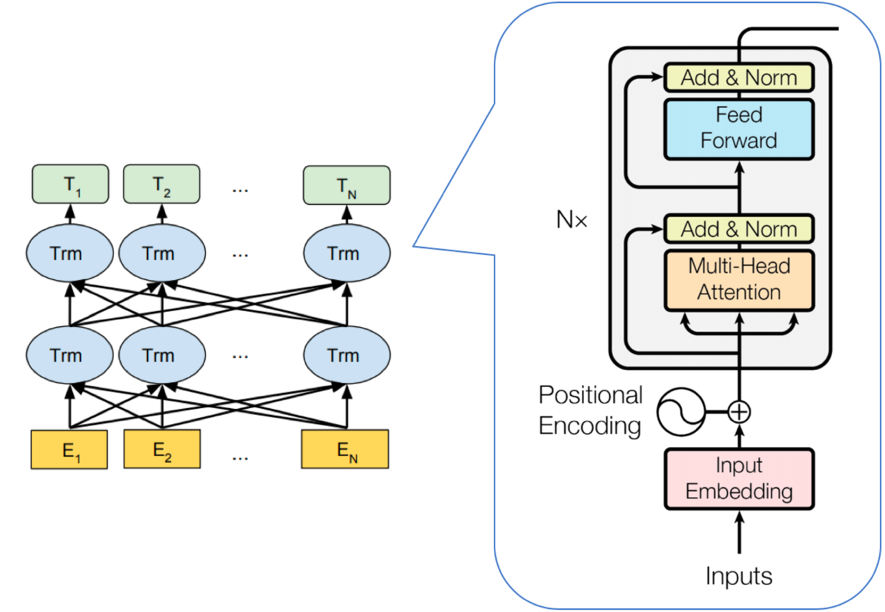
\includegraphics[width = 0.8\textwidth]{transformer.png}
	\caption{BERT以及Transformer Encoder部分结构图}
	\label{fig:transformer}
\end{figure}




基于BERT预训练模型的特征表示主要有两种方式:
一种是基于微调(Fine-turn)的方法,另一种是基于特征表示的方法。
在本章中使用的是基于微调的方法,使用本任务的数据集对预训练模型进行微调
,使预训练模型更加适合我们的任务。

给定一个句子和对应的标签,用$S=(w_1,w_2,…,w_n)$表示该句子,n表示该句子的长度。
在送入到预训练模型之前首先需要在每一个句子前加入[CLS]标志位
,并且在句子末尾添加[SEP]标志位。
[CLS]标签和[SEP]标签都是BERT的保留关键词
,其中[CLS]对应位置的最终输出代表了句子S的信息聚合,
也就是整个句子的表征向量,本节后续使用该向量进行分类;
[SEP]用于句子的分隔,主要在NSP任务中使用,本任务中只作为句子的结束符。
[CLS]位置的输出是一个768维的向量,将其输入到一个前馈神经网络中进行分类。


\section{恶意代码文本能力分类}
本章主要讲述句子级的恶意代码文本分类方法。针对数据集过小的问题,本章根据SnowBall的思想,
对数据进行了数据增强,扩充了数据,使得模型效果有了较大的提升。
本章提出了基于图卷积神经网络的模型,整体模型结构如图所示。
模型利用静态图的先验知识来对句子和单词做嵌入,然后利用基于注意力机制的全局动态图结构,
动态学习节点之间的拓扑结构,使其更加贴合下游任务,最后输入到前馈神经网络进行分类,获得了不错的效果。

\subsection{基于SnowBall思想的数据增强}
如4.2节所介绍的,数据集的规模较小,在训练中容易造成过拟合等问题。
为了解决这个问题,本章结合SnowBall的思想,对数据集进行了数据增强。
SnowBall的核心思路是一个迭代过程,首先使用原始数据集训练模型,对新的数据集行判断。
然后使用一定的方法来选取其中高置信度的新数据加入到训练集中再继续迭代,
从而达到增加数据集的目的,具体流程如图~\ref{fig:snowball}~所示。


\begin{figure}[htb]
	\centering
	\includegraphics[width = 0.9\textwidth]{SnowBall.png}
	\caption{SnowBall流程图}
	\label{fig:snowball}
\end{figure}

本节从Kaspersky、McAfee、Microsoft Security Response Center以及Github APT共享仓库等
地方收集恶意代码文本报告,一共收集了179个恶意代码文本报告。
部分恶意代码文本报告为PDF格式,无法直接使用,需要对其进行处理获取格式化的文本数据。
在获取到格式化的文本数据之后,我们首先需要判断句子中是否包含恶意能力的描述。
筛选出包含了描述恶意代码能力的句子之后,使用模型对这些句子打上标签,作为新的训练数据,
来达到扩充数据集的目的。数据增强的主要流程如图~\ref{fig:dataenhance}~所示。
\begin{figure}[htb]
	\centering
	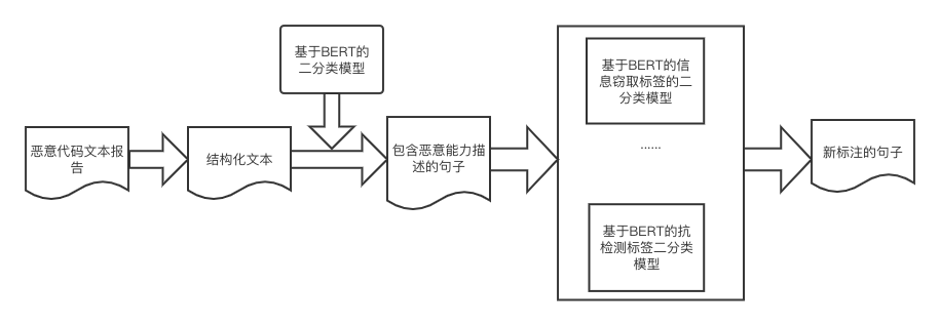
\includegraphics[width = 0.9\textwidth]{dataenhance.png}
	\caption{数据增强流程图}
	\label{fig:dataenhance}
\end{figure}

首先需要将PDF格式的APT报告转换成txt格式,这里使用PDFminer来进行转换。
由于不同PDF的格式排版存在较大差异存在大量转化后的文本有较多散乱文本需要进行处理,
如图~\ref{fig:pdf2txt}~所示。

\begin{figure}[htb]
	\centering
	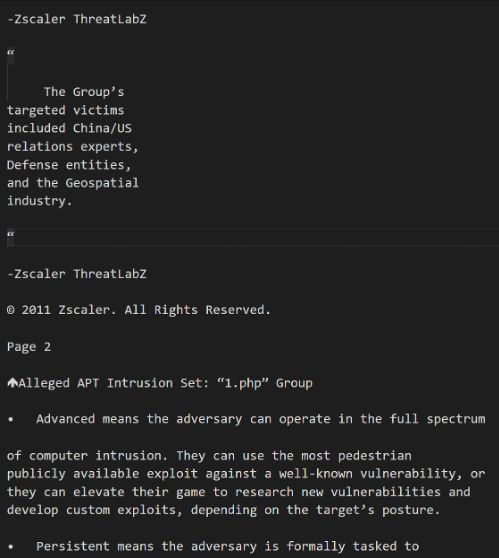
\includegraphics[width = 0.5\textwidth]{pdf2txt.png}
	\caption{pdf转换为txt之后的文本}
	\label{fig:pdf2txt}
\end{figure}

根据转化后的文本中存在的问题,本节构造了对应的规则来进行处理。
首先以空行为界限进行段落的划分,将文本细分方便后续处理。
由于PDF的排版问题,几乎所有的段落都存在较多的换行,因此我们将段落中的行进行拼接,
其中存在一种特殊情况也就是同一个单词之间使用“-”分割换行的情况需要单独处理。
考虑到文本中包含着大量的时间信息、组织信息、作者信息、页码标注等无用的短文本,
我们设置了一个长度阈值来对段落进行过滤,有效剔除了这些无用文本。处理后的结果如图~\ref{fig:ruletext}~示。

\begin{figure}[htb]
	\centering
	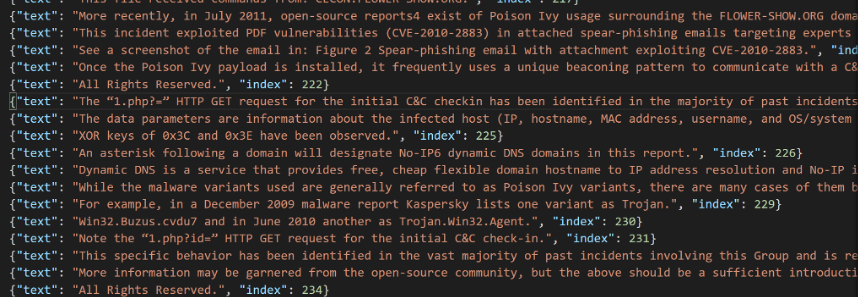
\includegraphics[width = 0.9\textwidth]{ruletext.png}
	\caption{处理后的文本}
	\label{fig:ruletext}
\end{figure}

在构建了结构化的文本数据之后,需要判断该句子是否描述了恶意能力以及描述了何种能力。
这里使用预训练模型BERT来判断其标签。
在原训练数据的基础上,我们分别针对七种标签训练了七个独立的二分类模型,每个模型判断句子是否描述了对应的恶意能力。

为了提高新数据的准确性,模型主要以精确率(Precision)来作为模型选择的标准,精准率的公式如(~\ref{p}~)所示。
提高精准率能够保证正样本的准确性,但是会牺牲正样本的数量,使得部分正样本被判定为负样本而被舍弃。
从数据增强的角度来说,这是最合理的选择。

\begin{equation}
	\label{p}
	\text{Precision}=\frac{TP}{TP+FP}
\end{equation}

训练阶段对超参数进行调整,使模型性能达到参数范围内的最优。
再分别对各个模型结果判断设置阈值,
使得模型判断为正样本的逻辑从模型输出的正样本的概率大于负样本
转化为除了满足模型输出的正样本的概率大于负样本的条件以外
还需要正样本的置信度大于阈值。置信度的设置使得模型在验证集上的准确率达到100\%的阈值。
在训练完模型之后再对新的文本数据进行标注,获得了1814条新的数据,将数据集扩展了接近一倍。

\subsection{基于图神经网络的恶意代码文本分类模型}
该模型主要由基于图卷积神经网络的编码层以及基于自注意力机制的全局图和一个前馈神经网络构成,
整体结构如图所示。

图卷积神经网络能够捕捉句子中的图结构,可以根据文本的特点来进行构图。
考虑到恶意代码文本中存在大量的专业名词具有较多的信息,例如CVE,
在one-hot编码的的处理方法会将其当作一个普通的单词节点进行处理;
而在GloVe等预训练embedding模型中,将无法找到对应的embedding从而对其进行随机生成或者用特定值,
这样做会丢失其中的信息。
为了解决这个问题,引入了外部知识节点,通过外部知识来对其进行解释,保证专业名词节点能够不被忽略。

图中主要有三类节点,分别是句子节点、单词节点以及外部知识节点。
图中边主要采用共现的思路进行构筑。
图$\mathbf{G=(V,E)}$,$\mathbf{V}$代表节点的集合,$\mathbf{E}$代表边的集合。
句子集合$\mathbf{S}=\{s_1,…s_n\}$,其中$n$代表数据集中句子的个数,
单词集合$\mathbf{W}=\{w_1,…w_m\}$,其中$m$代表单词节点的个数,
外部知识集合$\mathbf{K}=\{k_1,…,k_l\}$,其中$l$代表外部知识的节点个数,
邻接矩阵$\mathbf{A} \in \mathbb{R}^{(n+l+m)×(n+l+m)}$记录了图中的所有边以及对应的权重,
当两个节点不存在边的时候,邻接矩阵$\mathbf{A}$对应的位置为0。

图中主要存在三类边:句子和单词之间的边,单词和单词之间的边以及单词和外部知识之间的边。
下面将分别介绍三种边的构建思路以及对应的权重赋予方法。

句子和单词之间的边采用包含关系来构建,即为当单词$w_i$出现在句子$s_j$中时候,构筑一条边。
句子和单词之间的边的权重采用改进后的词频-逆文档频率,
恶意句子词频-逆常规文档频率(Malware Sentence term Frequency-Inverse Normal Sentence Frequency,MSF-INSF)
来进行计算。
本章中使用的文本数据都是恶意代码文本中获取的句子,有着类似的主题,
因此在多个句子中出现的单词很可能也是重要程度高的词。
如果直接使用TF-IDF进行权重的计算会导致一些信息量较大的关键词的权重由于在多个句子中出现反而会被降低,
MSF-INSF是针对本任务对传统的TF-IDF计算方法进行改进,引入了外部常规文本数据。
通过分别计算单词在恶意代码句子中的出现频率以及在普通句子中的逆文档频率,
将两者的乘积作为边的权重,计算方法如下:
\begin{equation}
	\label{TF}
	MSF_i = \frac{\#S(w_i)}{\#S}
\end{equation}
\begin{equation}s
	\label{IDF}
	INSF_i = log\frac{\#N}{\#N(w_i)+1}
\end{equation}
\begin{equation}
	TF-IDF_i=TF_i \times IDF_i \times \alpha
\end{equation}

其中$w_i$表示恶意代码文本中的某一单词,
$\#S$表示恶意代码数据集中句子的个数,$\#S(w_i)$表示单词$w_i$出现的句子的个数,$\#N$表示外部常规文档的总句子个数,
$\#N(w_i)$表示恶意代码文本中的单词在外部文档中的出现次数。

单词之间的边通过对句子进行句法分析后获得的依存关系(Dependency Parsing)来进行构建。
依存关系能够捕捉单词之间的句法关系,并且缩短句子中的关键信息的距离。
同时依存关系是一组单词两两之间的关系,形式上适合用于构建单词之间的边。依存关系的例子如图~\ref{fig:dep}~所示。

\begin{figure}[htb]
	\centering
	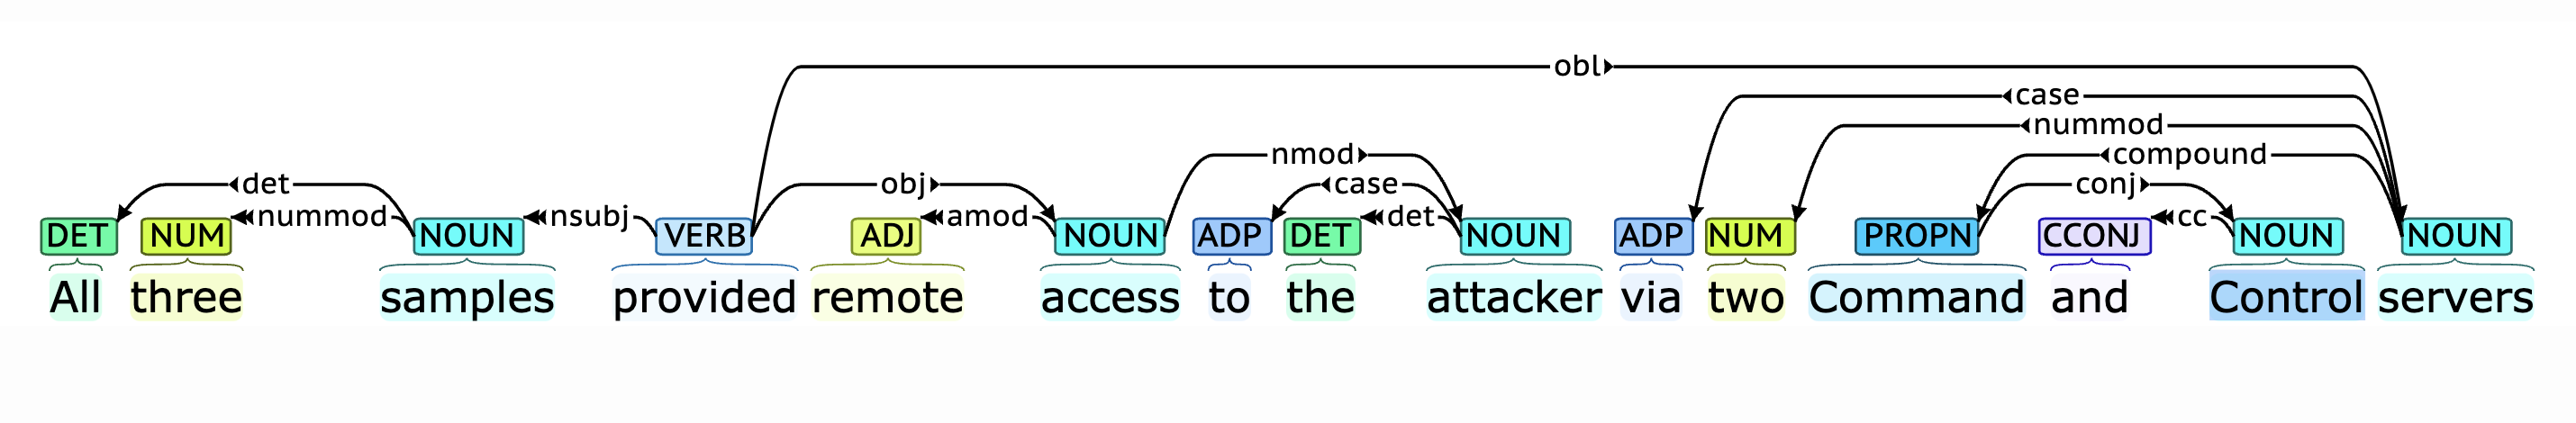
\includegraphics[width = 1\textwidth]{句法分析.png}
	\caption{依存关系例子}
	\label{fig:dep}
\end{figure}

单词与外部知识节点的边直接在外部知识与对应的专业名词的单词节点之间构建,权重设置为超参数。

模型静态图的构建算法如下所示:

\vspace{0.5cm}
\IncMargin{1em}
\begin{algorithm}[H]
\wuhao
\SetKwInOut{Input}{输入}
\SetKwInOut{Output}{输出}
\Input{句子集合$\mathbf{S}=\{s_1,s_2,...,s_n\}$,单词集合$\mathbf{W}=\{w_1,w_2,...,w_m\}$,外部知识$\mathbf{K}=\{w_x:k_1,w_y:k_2,...w_z:k_l\}$
TF-INDF权重矩阵$\mathbf{W}$以及句法依存树} 
\BlankLine 
\Output{静态图的邻接矩阵$\mathbf{A}$}
\BlankLine
句子和单词之间的边的构建\\
\For{$i in 1 \rightarrow m$ }{
	\For{$j in 1->n$}{
		\If{$w_i \in s_j $}{
			$\mathbf{A}_{i,n+l+j} \Leftarrow \mathbf{W}_{i,j}$
			}
	}
}
外部知识与单词之间的边的构建\\
\For{$i in \rightarrow l$}{
	$w_x \leftarrow \mathbf{K}[i]$\\
	$\mathbf{A}_{n+l+x,n+i} \Leftarrow \alpha$ 
}
单词之间的边的构建\\
\For{$i in 1 \rightarrow m $}{
	\For{$j in i \rightarrow m $}{
		\If{$(w_i,w_j)$ in dependency Tree}
		{
			$mathbf{A}_{i,j} \Leftarrow \mathbf{A}_{i,j} + 1 $
		}
	}
}
\textbf{return} \emph{$\mathbf{A}$}
\caption{恶意代码关联行为挖掘算法}
\label{a1} 
\end{algorithm}
\DecMargin{1em}
\vspace{0.5cm}


完成了基于句子结合以及语法依存关系的静态图的构建之后,将图送入到图卷积层进行运算。
首先为了防止在聚合过程中出现邻居节点多的节点会相比于其他节点有着更大的影响力的情况,
需要对邻接矩阵进行规范化,具体方法如下:
\begin{equation}
	\label{Dii}
	\mathbf{D}_{ii} = \sum_{j=0}^{n+l+m}\mathbf{A}_{ij}
\end{equation}
\begin{equation}
	\label{L}
	\mathbf{L} = \mathbf{D}^{-\frac{1}{2}} \mathbf{A} \mathbf{D}^{-\frac{1}{2}}
\end{equation}

其中$\mathbf{D}$表示邻接矩阵的度矩阵,对角线上元素表示对应位置节点的度,其余部分均为0。
在获得了拉普拉斯矩阵$\mathbf{L}$之后就可以进行图卷积运算,计算公式如下:

\begin{equation}
	\label{graphconver}
	\mathbf{H}^{i+1} = ReLU(\mathbf{LH}^i\mathbf{W}_i)
\end{equation}

其中$\mathbf{H}^i$表示上一层输出的节点特征,
最初的$\mathbf{H}^0=\mathbf{X}$,
此处$\mathbf{X}$的输入为所有节点的独热编码的矩阵。
$\mathbf{W}_i$为每层的可学习的参数,用于图聚合之后的结果进行线性变换。
如图/所示,K层图卷积层能够使得节点学习到对应的K阶段邻居。
由于本章中构建的静态图主要是由句子和单词节点构成,学习二阶邻居即可让句子之间相互学习。
此时再增加层数不仅会增加计算量,而且会导致图的节点同质化,使模型性能下降,具体的实验结果在4.7节中讲述。

通过基于静态图的图卷积神经网络之后,可以得到句子节点和单词节点的嵌入表示。
由于静态图是采用非监督算法,根据先验知识构建的,无法完全契合下游任务的需求。
这里采用基于注意力机制的全局图结构来动态学习不同节点之间边。
考虑到图中三类节点的性质,在句子和不相关单词之间添加边是不合理的,以及外部领域知识节点与不相关单词和句子之间
添加边也是不合理的。
因此这里在句子节点之间利用注意力机制来动态学习图的拓扑结构。
具体算法如下:
\begin{equation}
	\label{q}
	\mathbf{Q} = \mathbf{XW_Q}
\end{equation}
\begin{equation}
	\label{k}
	\mathbf{K} = \mathbf{XW_K}
\end{equation}
\begin{equation}
	\label{s}
	\mathbf{S} = Softmax(\frac{\mathbf{QK^T}}{\sqrt{d}})
\end{equation}
\begin{equation}
	\label{h}
	\mathbf{H=XS}
\end{equation}

其中$\mathbf{X}$表示句子节点的嵌入,$\mathbf{W_Q}$ ,$\mathbf{W_K}$是可训练的参数矩阵,
$\mathbf{Q}$,$\mathbf{K}$分别代表Query矩阵和Key矩阵,d表示embedding的维度,用于对结果正则化,
$\mathbf{S}$为Attention计算之后的权重矩阵,$\mathbf{H}$为经过动态图的聚合之后的结果。

由于做全局Attention的时候自身到自身的权重也是通过自身的Query和Key计算获得的,
这样做可能会导致自身信息的丢失,违背了本意,因此参考了残差连接的思想添加skip connect。
\begin{equation}
	\label{resnet}
	\mathbf{E=[H\|X]}
\end{equation}
\begin{equation}
	\label{fnn}
	\text{Label} = argmax(Softmax(FFNN(\mathbf{E})))
\end{equation}

其中$\mathbf{E}$为残差连接的结果,为最终的句子嵌入表示。
之后将句子嵌入表示矩阵输入到一个前馈神经网络中(Feed Forward Neural Network,FFNN)进行线性变换,
输出的维度为n×7,其中n为句子的个数,7为标签数。
FFNN的输出输入到Softmax层,得到的即为各个标签的概率。

分类问题常用的失函数的是交叉熵,计算方式如下:
\begin{equation}
	\label{ce}
	Loss = -\sum_{i=0}^{C-1}y_ilog(p_i)
\end{equation}

其中C表示类别的总数,$y_i$表示标签的one-hot表示,
当i为对应的类别时$y_i$为1,其余均为0,$p_i$是模型的softmax层的输出表示模型判断其类别为i的概率。

由于本章使用的数据如4.2节所示存在样本分布不均衡的问题,因此采用FocalLoss来作为损失函数,
FocalLoss的思想是让模型更多关注样本数量少的类别以及难度大的类别。难度大指的是模型预测的结果与
实际结果的差距较大。
Focalloss的实现方法在交叉熵的基础上添加了$\alpha$和$\gamma$两个超参数来
分别对应样本的权重和难度系数。
在多分类中的实现如下所示:
\begin{equation}
	\label{focalloss}
	\text{FocalLoss} = -\sum_{i=0}^{C-1}y_i \alpha_i (1-p_i)^{\gamma}log(p_i)
\end{equation}

其中$\alpha_i$ 表示类别i的权重,该参数越大表示对该类别的样本重视程度越大,反之则表示重视程度低,$\gamma$表示难度系数,
该参数越大表示对难度大的样本重视程度越大。当$\alpha_i$全为1,$\gamma$为0的时候退化为交叉熵。
本节中$\gamma$参数采用经验值1,$\alpha$参数根据训练集中样本的数量来产生,计算方法如(~\ref{aplha_work}~)所示。
其中$N_i$表示i类样本的数量,$N$表示总的样本数量。
\begin{equation}
	\label{aplha_work}
	\alpha_i = \frac{N_i}{N}
\end{equation}

\section{恶意代码家族画像构建}
从前面几个小结中可以获得恶意代码的家族能力以及家族共同行为,
因此将两个部分组合即可得到恶意代码的家族画像。

本小节在恶意代码个体画像的基础上进行,整体流程如图所示。

恶意代码个体行为存在不同的混淆机制,这就导致了同一家族的不同个体之间存在着行为的差异。
考虑到同一家族的根本恶意目的相同,个体的行为无论如何混淆都无法避开为了达到恶意目的所产生的行为,
因此本节对恶意代码个体的行为进行聚合,来获得恶意代码家族的行为。
本节采用基于关联规则的算法来对恶意代码动态行为进行聚合。
关联规则用于发现数据变量之间有意义的关系,例如当事件AB总是同时发生,那么两个事件可能是关联的。
在恶意代码行为中同理,当同一家族的样本中总是出现固定几个行为,这些行为很可能就是该家族的关键行为。
在此基础上还提出了基于能力标签的聚合进一步提升算法的准确性。

首先根据恶意代码个体画像的家族标签进行分组,将同家族的个体画像放在一起。
然后对个体样本的画像进行求并集,并且统计每个条目出现的个数。
获得了同一家族的所有个体样本的行为并集之后,对条目做Min-Max归一化,方法如式子(~\ref{minmax}~)所示。

\begin{equation}
	\label{minmax}
	N_{new} = \frac{N_i-N_{min}}{N_{max}-N_{min}}
\end{equation}

其中$N_i$为其中某项条目出现的次数,$N_min$是该家族中所有条目出现次数最多的数字,
$N_max$则是该家族所有条目中出现次数最多的数字。

完成了归一化之后需要设置一个阈值$\beta$来进行筛选,
当出现的比例小于$\beta$的时候则视为噪声舍弃,
当出现的比例大于$\beta$的时候则认为是该家族的共同行为。

考虑到部分行为会在大部分的代码中出现,因此需要再对这些行为进行处理。
这里采用了能力标签来进行整合。
由于恶意代码的行为本质上是为了实现其能力而产生的,
因此根据家族的能力标签再做一次聚合操作可以筛选出能力对应的恶意代码行为。

首先根据能力标签来进行划分,具有相同能力标签的家族样本放到同一集合,然后
在对行为进行统计,做特征筛选。
完成能力行为对应的筛选之后再对各个能力标签之间做差集,筛选出该能力对应的行为。


\section{实验结果与分析}

\subsection{实验设计}
这类分别针对两个子任务设计了实验。针对恶意代码语句相关性判别任务,由于与SemEval-2018中的数据一致,因此与
该任务中提交的方案进行对比。
针对恶意代码句子能力分类任务,主要设计了三组实验,第一组将本章提出的模型与现有的基线方法进行对比,证明模型的有效性。
第二组为消融实验,主要用于验证模型各个部分以及预处理和数据增强的效果。 第三组为模型结构的部分设计对比例如GCN的层数对比。


\subsection{恶意代码语句相关性判别实验结果}
该任务中使用的是以BERT预训练模型为主的模型,主要参数如表~\ref{tab:bert}~所示
\begin{table}[htb]
	\renewcommand{\arraystretch}{1.3}
	\caption{BERT预训练模型}
	\label{tab:bert}
	\vspace{0.5em}\centering\wuhao
	\setlength{\tabcolsep}{12mm}{
	\begin{tabular}{c c}
		\toprule[1.5pt]  超参数 & 值 \\
		\midrule[1pt] 
		学习率 & 1e-5 \\
		优化器 & AdamW \\
		Mini-Batch大小 & 32 \\
		Dropout & 0.3 \\ 	
		Warmup轮数比例 & 0.1 \\ 
		
		\bottomrule[1.5pt] 
	\end{tabular}}
\end{table}

基于BERT预训练模型与SemEval-2018中提交的方案的对比如表~\ref{tab:task1}~所示。
\begin{table}[htb]
	\renewcommand{\arraystretch}{1.3}
	\caption{恶意代码句子相关性判别任务结果}
	\label{tab:task1}
	\vspace{0.5em}\centering\wuhao
	\begin{tabular}{c c c c c }
		\toprule[1.5pt]  & Precision & Recall & F1 & Acc \\
		\midrule[1pt] 
		SVM baseline & 49.55 & 62.22 & 55.17 & 80.58 \\
		NB baseline  & 38.17 & $\mathbf{78.89}$ & 51.45 & 78.32 \\
		Random uniform baseline & 16.09 & 56.67 & 25.06 & 50.65 \\
 		Random stratified baseline & 11.45 & 16.67 & 13.57 & 69.09 \\
		GLoVe+BiLSTM\cite{RN102}& 47.76 & 71.11 & 57.14 & 84.47 \\
		CRF+NB\cite{RN103} & 49.59 & 66.67 & 56.87 & 85.28 \\
		BiLSTM+CNN+CRF\cite{RN104} & 53.57 & 50.00 & 51.72 & 86.41 \\
		Digital Operatives\cite{RN105} & 39.31 & 75.56 & 51.71 & 79.45 \\
		GLoVe+CNN\cite{RN106} & 38.46 & 72.22 & 50.19 & 79.13 \\
		word2vec-MLP\cite{RN101} & 11.14 & 43.33 & 17.73 & 41.42 \\
		% NanshanNLP & 13.56 & 17.78 & 15.38 & 71.52 \\
		BERT+FFNN & $\mathbf{78.00}$  & 72.00  &  $\mathbf{75.00}$ & $\mathbf{90.00}$\\
		% LowPick+BERT+FFNN & 78.70 & 77.55 & 77.98 & 77.55 \\
		\bottomrule[1.5pt] 
	\end{tabular}
\end{table}
总的来说,基于BERT的模型在其中获得了最好的效果。



\subsection{恶意代码句子能力分类任务}
首先是对恶意代码句子能力分类的结果。由于数据集不是公共数据集,因此采用了诸多基准模型进行对比。
其中机器学习算法包括逻辑回归(Logistic Regression,LR),支持向量机(Support Vector Machine,SVM),XGBoost,Light GBM;
基于深度学习算法包括长短期记忆网络(Long short-term Memory,LSTM)、预训练模型BERT以及基于BERT的一些算法。
主要指标有Weighted-F1,Macro-F1,Acc,结果如表所示~\ref{tab:mainmultclass}~。 
\begin{table}[htb]
	\renewcommand{\arraystretch}{1.3}
	\caption{恶意代码句子能力分类实验结果}
	\label{tab:mainmultclass}
	\vspace{0.5em}\centering\wuhao
	\begin{tabular}{c c c c c c }
		\toprule[1.5pt]  & Weighted-F1 & Macro-F1 & Acc \\
		\midrule[1pt] 
		MC-LR & 56.45 & 47.46 & 57.50 \\
		PMC-LR & 56.77 & 46.61 & 56.50 \\
		EMC-LR & 56.43 & 49.00 & 57.50 \\
		PEMC-LR & 55.73 & 48.97 & 56.00 \\
		MC-SVM & 57.08 & 48.59 & 57.00 \\
		PMC-SVM & 57.50 & 49.65 & 57.50 \\
		EMC-SVM & 53.51 & 46.71 & 54.00 \\
		PEMC-SVM & 56.61 & 49.17 & 56.00 \\
		MC-xgb & 55.72 & 43.95 & 57.33 \\
		PMC-xgb & 56.04 & 43.79 & 57.33 \\
		EMC-xgb & 60.27 & 50.70 & 61.66 \\
		PEMC-xgb & 60.54 & 52.10 & 61.66 \\
		MC-lgbm & 45.86 & 31.05 & 50.00 \\
		PMC-lgbm & 50.68 & 39.46 & 53.50 \\
		EMC-lgbm & 50.10 & 39.63 & 52.50 \\
		PEMC-lgbm & 55.14 & 45.72 & 56.50 \\
		MC-BiLSTM & 65.47 & 52.36 & 66.50 \\
		PMC-BiLSTM & 66.34 & 53.98 & 66.50 \\
		EMC-BiLSTM & 64.26 & 52.13 & 65.00 \\
		PEMC-BiLSTM & 68.67 & 56.32 & 70.00 \\
		MC-LSTM & 62.57 & 50.41 & 62.50 \\
		PMC-LSTM & 65.15 & 50.78 & 67.00 \\
		EMC-LSTM & 64.78 & 53.02 & 65.00 \\
		PEMC-LSTM & 67.95 & 59.44 & 67.00 \\
		MC-BERT-FFNN & 61.58 & 47.21 & 64.00 \\
		PMC-BERT-FFNN & 70.13 & 62.30 & 70.00 \\
		EMC-BERT-FFNN & 72.22 & 62.94 & 72.50 \\
		PEMC-BERT-FFNN & 69.27 & 55.85 & 70.00 \\
		MC-BERT-CNN & 69.26 & 55.80 & 71.00 \\
		PMC-BERT-CNN & 71.40 & 62.50 & 71.50 \\
		EMC-BERT-CNN & 67.01 & 53.93 & 68.00 \\
		PEMC-BERT-CNN & 71.62 & 61.81 & 71.52 \\
		MC-BERT-RNN & 70.51 & 55.25 & 72.00 \\
		PMC-BERT-RNN & 64.30 & 47.68 & 67.00 \\
		EMC-BERT-RNN & 72.35 & 63.32 & 72.50 \\
		PEMC-BERT-RNN & 67.21 & 51.69 & 67.50 \\
		MC-KG-SDGCN & 70.61 & 65.00 & 70.50 \\
		PMC-KG-SDGCN & 68.50 & 60.14 & 69.00 \\
		EMC-KG-SDGCN & 73.15 & 66.02 & 73.50 \\
		PEMC-KG-SDGCN & 74.64 & 69.06 & 74.50 \\
		\bottomrule[1.5pt] 
	\end{tabular}
\end{table}

其中MC(Malware Capability)表示原始数据,PMC(Preprocessed Malware Capability)表示针对恶意代码文本
的特点预处理之后的数据,EMC(Enhance Malware Capability)表示经过SnowBall增强之后的数据,
PEMC(Preprocessed Enhance Malware Capability)表示经过预处理以及数据增强之后的数据。
从表示可以看出,KG-SDGCN的表现超过了其他的对比模型,与其他的最好的结果相比,ACC提升了,Macro-F1提升了,
这表明本章提出的模型可以很好处理恶意代码相关文本,达到更好的性能。KG-SDGCN的具体的各个能力类别的表现如表所示。

\begin{table}[htb]
	\renewcommand{\arraystretch}{1.3}
	\caption{KG-SDGCN对各个类别的表现情况}
	\label{tab:task1}
	\vspace{0.5em}\centering\wuhao
	\begin{tabular}{c c c c }
		\toprule[1.5pt]  & Precision & Recall & F1 \\
		\midrule[1pt] 
		0   &  72.73  &  70.59  &  71.64   \\
		1   &  27.27  &  27.27  &  27.27   \\  
		2   &  69.57  &  80.00  &  74.42   \\     
		3   &  82.35  &  80.00  &  81.16   \\     
		4   &  82.50  &  78.57  &  80.49    \\    
		5   &  61.90  &  76.47  &  68.42    \\    
		6   &  100.0  &  66.67  &  80.00    \\     
		\bottomrule[1.5pt] 
	\end{tabular}
\end{table}

其中可以看到KG-SDGCN在2类的表现较差。

\subsection{消融实验}
本节主要用于评估模型各个部分的影响。
首先对比KG-SDGCN的各个部分对结果的影响。
结果如表所示


其次对比不同数据处理方法对模型性能的影响,如上节所示,本章主要有针对恶意代码文本的预处理方法以及基于SnowBall思想
的数据增强方法,一共衍生了ME,EMC,PMC以及PEMC四种数据。
图~\ref{fig:datadiff}~对四类数据在不同的模型下的表现进行对比。

\begin{figure}[h]
	\centering
	\subfigure[GloVe-LR]{
		\begin{minipage}[t]{0.27\linewidth}
			\centering
			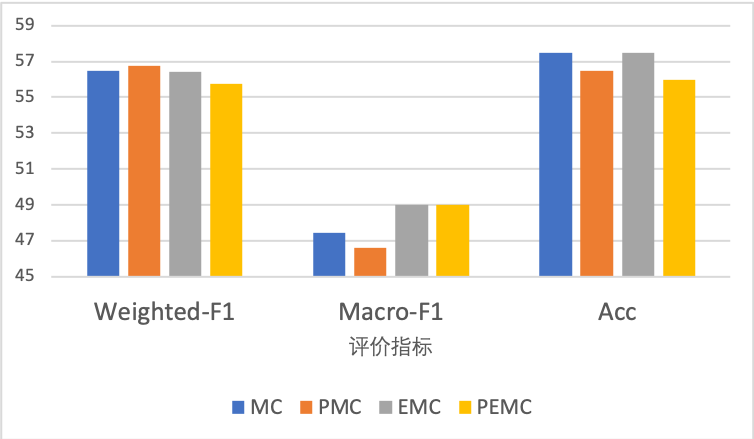
\includegraphics[width = 1.8in]{lr_data.png}
		\end{minipage}
	}
	\quad
	\subfigure[GLoVe-SVM]{
		\begin{minipage}[t]{0.27\linewidth}
			\centering
			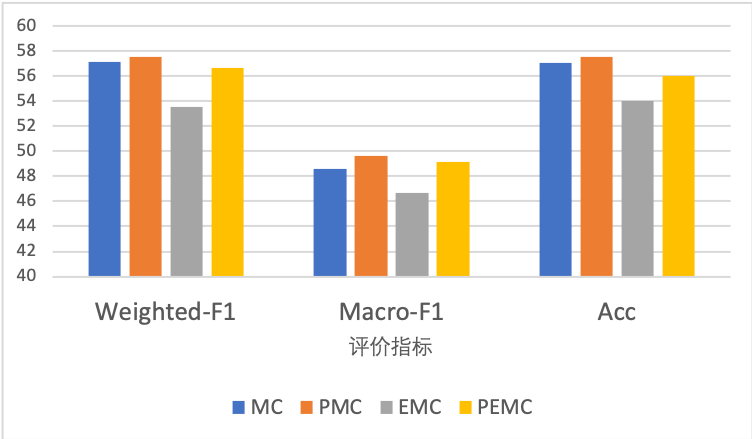
\includegraphics[width = 1.8in]{SVM_data.png}
		\end{minipage}
	}
	\quad
	\subfigure[GLoVe-XGB]{
		\begin{minipage}[t]{0.27\linewidth}
			\centering
			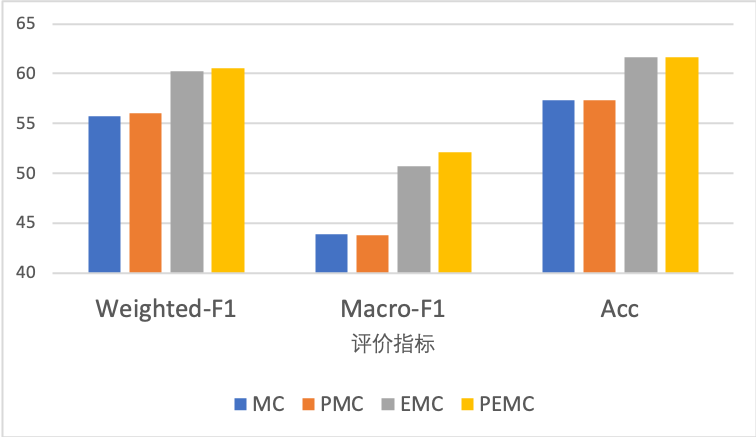
\includegraphics[width = 1.8in]{xgb_data.png}
		\end{minipage}
	}
	\subfigure[GLoVe-LGBM]{
		\begin{minipage}[t]{0.27\linewidth}
			\centering
			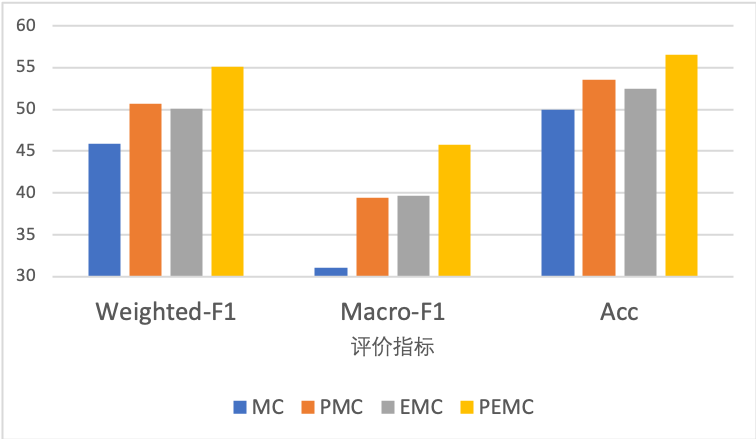
\includegraphics[width = 1.8in]{lgbm_data.png}
		\end{minipage}
	}
	\quad
	\subfigure[GLoVe-LSTM]{
		\begin{minipage}[t]{0.27\linewidth}
			\centering
			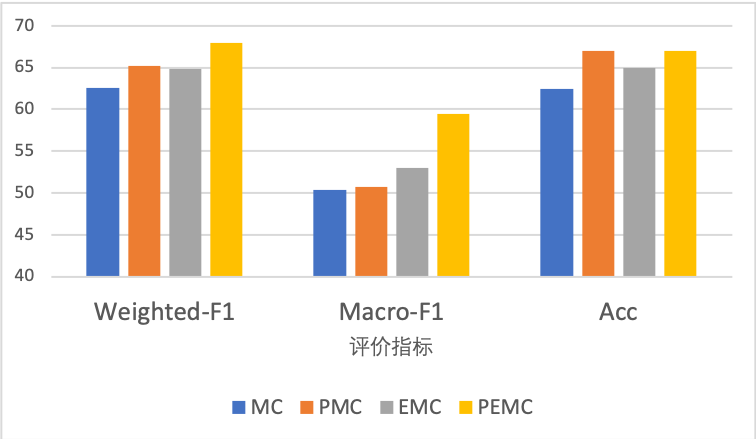
\includegraphics[width = 1.8in]{lstm_data.png}
		\end{minipage}
	}
	\quad
	\subfigure[GLoVe-BiLSTM]{
		\begin{minipage}[t]{0.27\linewidth}
			\centering
			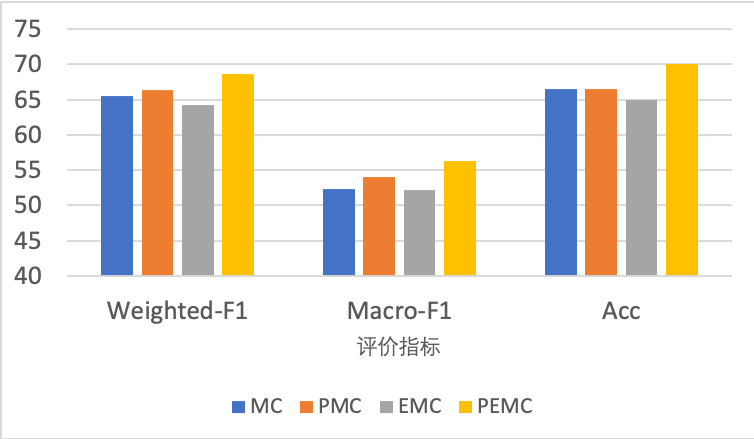
\includegraphics[width = 1.8in]{bilstm_data.png}
		\end{minipage}
	}
	\subfigure[BERT-FFNN]{
		\begin{minipage}[t]{0.27\linewidth}
			\centering
			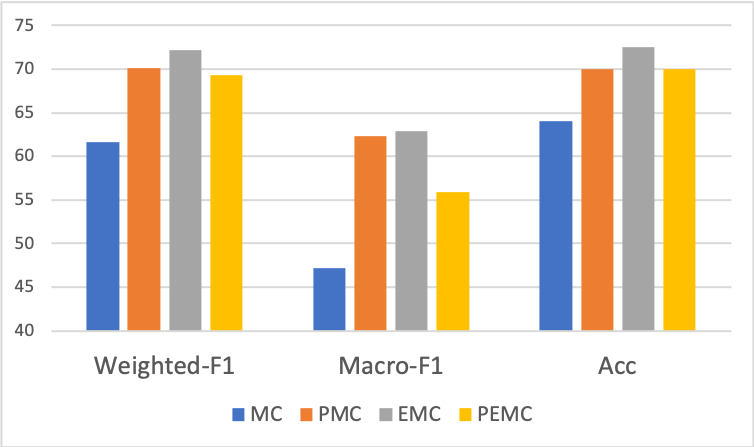
\includegraphics[width = 1.8in]{bert_ffnn.png}
		\end{minipage}
	}
	\quad
	\subfigure[BERT-CNN]{
		\begin{minipage}[t]{0.27\linewidth}
			\centering
			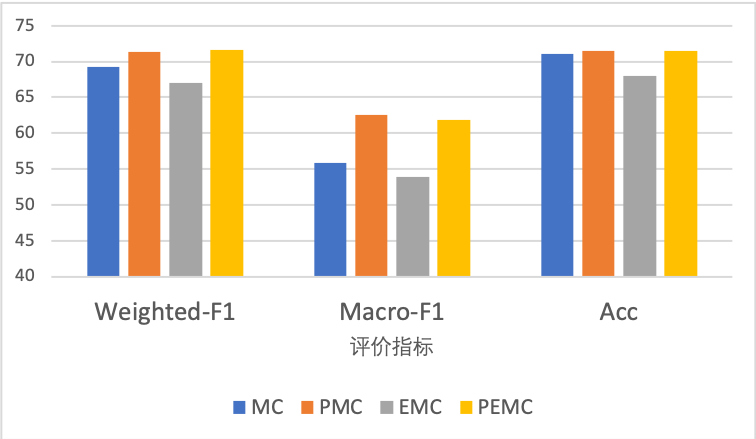
\includegraphics[width = 1.8in]{bert_cnn_data.png}
		\end{minipage}
	}
	\quad
	\subfigure[BERT-RNN]{
		\begin{minipage}[t]{0.27\linewidth}
			\centering
			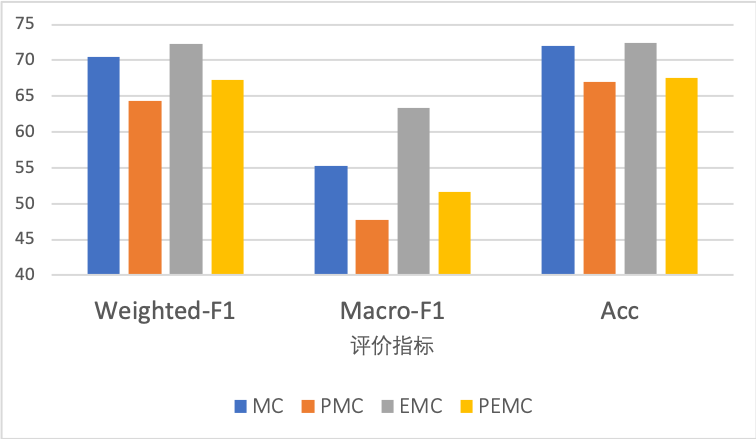
\includegraphics[width = 1.8in]{bert_rnn_data.png}
		\end{minipage}
	}
	\subfigure[KG-SDGCN]{
		\begin{minipage}[t]{0.27\linewidth}
			\centering
			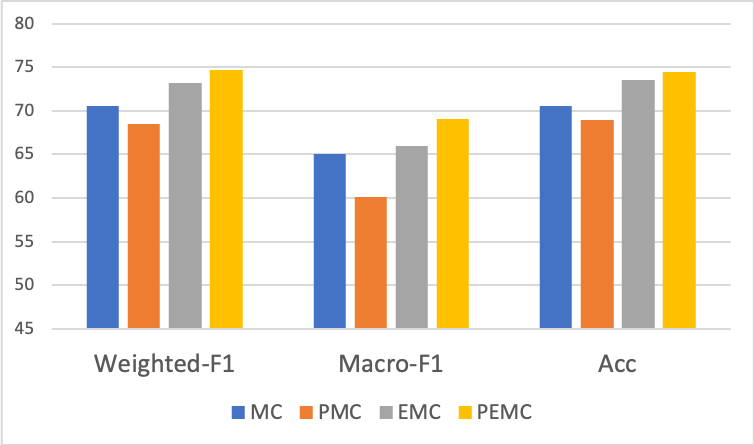
\includegraphics[width = 1.8in]{kg_sdgcn_data.png}
		\end{minipage}
	}
	\caption{模型在四种数据中的表现}
	\label{fig:datadiff}
\end{figure}

从图中可以看到,总的来说本章提出的针对恶意代码文本的预处理方法和基于SnowBall思想的数据增强方法获得了
预期的效果,数据增强的提升相对更多。



\subsection{模型部分参数影响对比}
本节主要对模型的部分结构相关参数进行对比。首先是静态图卷积部分的卷积层数对比,结果如表所示。
由于图卷积的性质可知,图卷积的层数对应节点可学到的邻居的阶数,理论上层数越多节点可以学到更多的
信息,但是实际上过多的层数会导致节点的信息同质化,反而降低质量。

动态图中多头Attention的头数的对比。在Attention机制中,多头可以用于学习任务中不同的特点。














